\subsubsection{Ý tưởng}
Quick Sort là thuật toán hoạt động bằng cách chia mảng thành hai phần dựa vào pivot (phần tử chốt) được chọn. Một bên bao gồm các giá trị nhỏ hơn pivot, bên còn lại chứa các giá trị lớn hơn pivot. Quick Sort sẽ được gọi đệ quy trên từng phần cho đến khi không thể chia nhỏ hơn nữa, sau đó mảng sẽ được sắp xếp.\cite{fasha2021comparative}

\subsubsection{Mã giả}
\begin{algorithm}[H]
\caption{Quick Sort (Choose middle element as pivot)}
\begin{algorithmic}[1]
\Procedure{QuickSort}{$arr, n$}
    \State \textbf{Input:} Mảng $arr$ gồm $n$ phần tử
    \State \textbf{Output:} Mảng $arr$ được sắp xếp
    \State \Call{QuickSortRecursive}{$A, 0, n - 1$}
\EndProcedure

\Procedure{QuickSortRecursive}{$arr, left, right$}
    \If{$left \geq right$}
        \State \textbf{return}
    \EndIf
    \State $pivot \gets$ \Call{Partition}{$arr, left, right$}
    \State \Call{QuickSortRecursive}{$arr, left, pivot - 1$}
    \State \Call{QuickSortRecursive}{$arr, pivot, right$}
\EndProcedure

\Procedure{Partition}{$arr, left, right$}
    \State $pivot \gets arr[\frac{left + right}{2}]$
    \State $i \gets left, j \gets right$

    \While{$i \leq j$}
        \While{$arr[i] < pivot$}
            \State $i \gets i + 1$
        \EndWhile
    
        \While{$arr[j] > pivot$}
            \State $j \gets j - 1$
        \EndWhile
    
        \If{$i \leq j$}
            \State \textbf{swap} $arr[i]$ \textbf{and} $arr[j]$
            \State $i \gets i + 1$
            \State $j \gets j - 1$
        \EndIf
    \EndWhile
    \State \textbf{return} $i$
\EndProcedure
\end{algorithmic}
\end{algorithm}

\subsubsection{Ví dụ}

\begin{figure}[H]
    \centering
    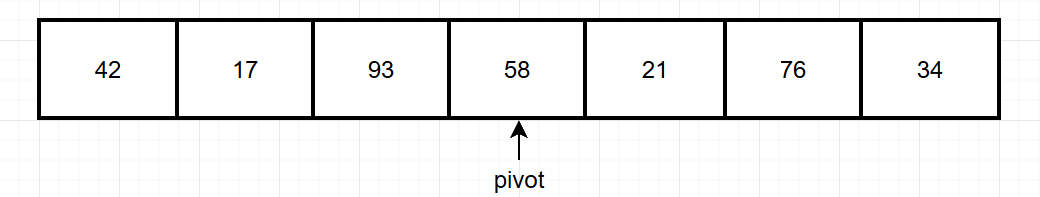
\includegraphics[width=1\linewidth]{img/quick_sort/1.png}
    
    \vspace{0.5cm}
    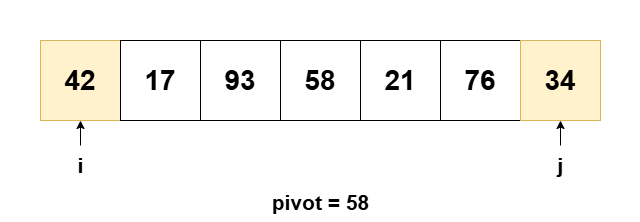
\includegraphics[width=1\linewidth]{img/quick_sort/2.png}
    \vspace{0.5cm}
    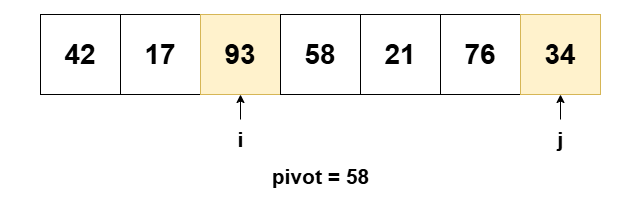
\includegraphics[width=1\linewidth]{img/quick_sort/3.png}
    \vspace{0.5cm}
    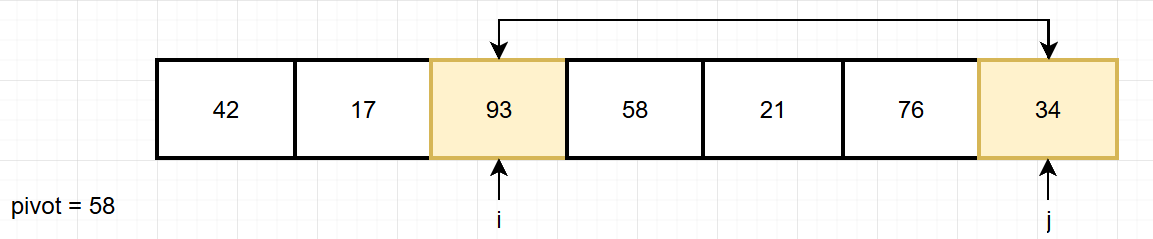
\includegraphics[width=1\linewidth]{img/quick_sort/4.png}
    \vspace{0.5cm}
    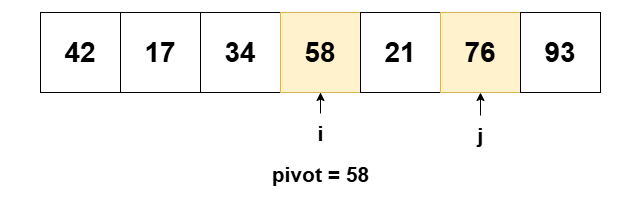
\includegraphics[width=1\linewidth]{img/quick_sort/5.png}
    \caption{Các bước chạy - 1}
\end{figure}

\begin{figure}[H]
    \centering
    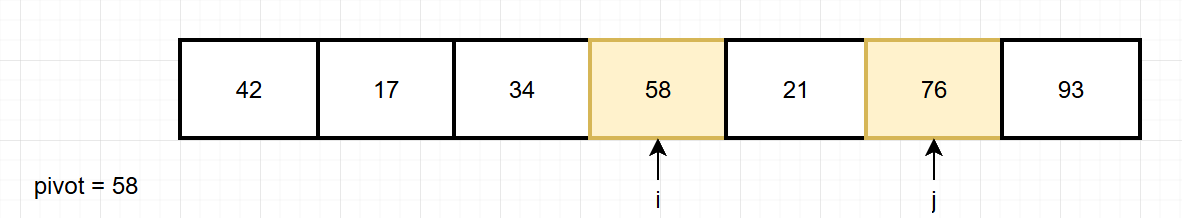
\includegraphics[width=1\linewidth]{img/quick_sort/6.png}
    
    \vspace{0.5cm}
    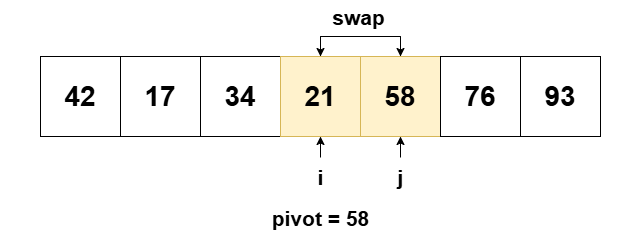
\includegraphics[width=1\linewidth]{img/quick_sort/7.png}
    \vspace{0.5cm}
    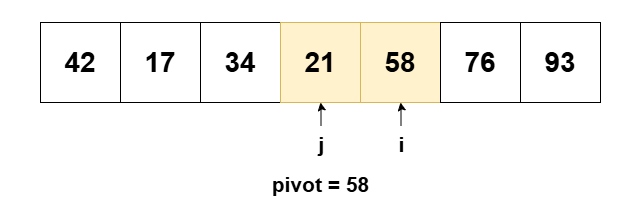
\includegraphics[width=1\linewidth]{img/quick_sort/8.png}
    \vspace{0.5cm}
    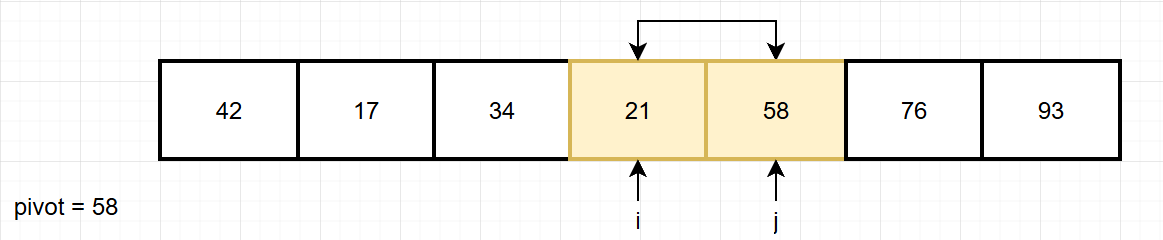
\includegraphics[width=1\linewidth]{img/quick_sort/9.png}
    \vspace{0.5cm}
    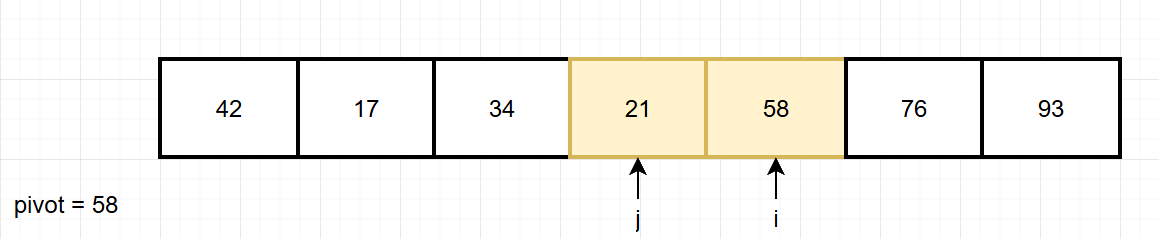
\includegraphics[width=1\linewidth]{img/quick_sort/10.png}
    \caption{Các bước chạy - 2}
\end{figure}

Ta sẽ gọi đệ quy lên mảng $[42,17,34,21]$ và $[58, 76,93]$ và thực hiện hoàn toàn tương tự các bước trên ta sẽ thu được mảng $[17, 21, 34, 42, 58, 76, 93]$ đã được sắp xếp.

\subsubsection{Độ phức tạp}
\begin{itemize}
    \item[\textbf{--}]Độ phức tạp về thời gian:
        \begin{itemize}
            \item[$\bullet$] \textbf{Best Case:} $O(n \cdot \log{n})$ 
            \item[$\bullet$] \textbf{Average Case:}  $O(n \cdot \log{n})$
            \item[$\bullet$] \textbf{Worst Case:}  $O(n^2)$
        \end{itemize}
    \item[\textbf{--}]Độ phức tạp về không gian: $O(\log{n})$ 
    \item[\textbf{--}]Tính ổn định: Không ổn định
\end{itemize}

